\section{Danh mục minh chứng}
Kho bàn giao sử dụng nhánh main. Đường dẫn ứng dụng tính từ \code{code/booking_classroom/}, backend từ \code{code/booking-server/}, báo cáo từ \code{docs/reports/final/LTUD/}; các đường dẫn khác tính từ gốc repository.
{\tabletext\renewcommand{\arraystretch}{1.04}\begin{longtable}{>{\raggedright\arraybackslash}p{\dimexpr0.19\textwidth-2\tabcolsep\relax}>{\raggedright\arraybackslash}p{\dimexpr0.45\textwidth-2\tabcolsep\relax}>{\raggedright\arraybackslash}p{\dimexpr0.36\textwidth-2\tabcolsep\relax}}
\caption{Hồ sơ bàn giao và vị trí}\label{tab:artifacts}\\
\toprule \textbf{Hạng mục} & \textbf{Vị trí / liên kết} & \textbf{Ghi chú}\\\midrule
\endfirsthead
\multicolumn{3}{l}{\small Hồ sơ bàn giao và vị trí (tiếp)}\\
\toprule \textbf{Hạng mục} & \textbf{Vị trí / liên kết} & \textbf{Ghi chú}\\\midrule
\endhead
\bottomrule\endlastfoot
Kho mã nguồn & \href{https://github.com/xwomen1/classroom-booking/tree/main}{GitHub: xwomen1/classroom-booking, nhánh main}. & Ứng dụng, backend, kiểm thử và tài liệu.\\\addlinespace[1.5pt]
README & Gốc repository: \code{README.md}; ứng dụng và backend: \code{README.md} tại từng thư mục. & Phụ thuộc, cấu hình, build và cài Android; Java/Maven, H2.\\\addlinespace[1.5pt]
Mã kiểm thử & Ứng dụng: \code{__tests__/}, \code{quality-tests/}, \code{src/modules/auto_approval/__tests__/}. & Bộ kiểm thử và cấu hình chạy riêng.\\\addlinespace[1.5pt]
Báo cáo kiểm thử & Ứng dụng: \code{quality-tests/BAO_CAO_KIEM_THU.md}; \code{evidence/device-verification.txt}. & Kết quả tự động, tích hợp H2 và kiểm tra Android.\\\addlinespace[1.5pt]
Hồ sơ thực nghiệm & Báo cáo: \code{minh_chung/kiem_thu/README.md}. & Môi trường, 50 ca app/398 quality/5 quyền thông báo; 6 ca Android, ảnh/XML và log.\\\addlinespace[1.5pt]
Nghiệm thu hệ thống & Báo cáo: \code{minh_chung/kiem_thu/nghiem_thu_he_thong.md}. & Kết quả vận hành ứng dụng và SmartLock do nhóm xác nhận.\\\addlinespace[1.5pt]
Ảnh giao diện & Báo cáo: \code{Hinhve/*hien_tai.png}; ảnh Android trong hồ sơ thực nghiệm. & Minh họa các chức năng tại Chương~\ref{chap:implementation}.\\\addlinespace[1.5pt]
Sơ đồ thiết kế & Gốc: \code{design/RoomHub_design.drawio}; báo cáo: \code{Hinhve/design/roomhub_bao_cao.drawio}. & Nghiệp vụ, kiến trúc, dữ liệu và trình tự xử lý.\\\addlinespace[1.5pt]
Bản chạy thử & Ứng dụng: \code{android/app/build/outputs/apk/release/app-release.apk} sau build. & Cài Android theo mục 4.7; chọn local/REST theo môi trường.\\\addlinespace[1.5pt]
Thống kê đóng góp & Báo cáo: \code{minh_chung/thong_ke_git.json}; \code{minh_chung/thong_ke_git.py}. & Số liệu quy thuộc dòng mã và script tái lập.\\\addlinespace[1.5pt]
\end{longtable}}

\Needspace{24\baselineskip}
\section{Kịch bản trình diễn 3--7 phút}
Kịch bản sử dụng bản Android đã cấu hình local hoặc REST, tài khoản user/admin, phòng khả dụng và hạn mức còn đủ. Luồng SmartLock sử dụng token hợp lệ và khóa đã gắn đúng phòng. Bảng~\ref{tab:demo} tổng hợp thao tác và trạng thái đầu ra dự kiến trong 3--7 phút.
{\tabletext\renewcommand{\arraystretch}{1.04}\begin{longtable}{>{\raggedright\arraybackslash}p{\dimexpr0.18\textwidth-2\tabcolsep\relax}>{\raggedright\arraybackslash}p{\dimexpr0.44\textwidth-2\tabcolsep\relax}>{\raggedright\arraybackslash}p{\dimexpr0.38\textwidth-2\tabcolsep\relax}}
\caption{Kịch bản demo và kết quả mong đợi}\label{tab:demo}\\
\toprule \textbf{Bước / thời lượng} & \textbf{Nội dung} & \textbf{Kết quả mong đợi}\\\midrule
\endfirsthead
\multicolumn{3}{l}{\small Kịch bản demo và kết quả mong đợi (tiếp)}\\
\toprule \textbf{Bước / thời lượng} & \textbf{Nội dung} & \textbf{Kết quả mong đợi}\\\midrule
\endhead
\bottomrule\endlastfoot
1 / 30 giây & Giới thiệu bài toán và chế độ dữ liệu của bản chạy; đăng nhập user. & Hiển thị bảng điều khiển User và các chức năng đặt phòng.\\\addlinespace[1.5pt]
2 / 60--90 giây & Chọn phòng/giờ ngày mai trong cửa sổ cho phép, nhập mục đích, gửi yêu cầu. & Tạo PENDING khi tự duyệt tắt; lịch phòng phản ánh khung giờ đã giữ.\\\addlinespace[1.5pt]
3 / 60--90 giây & Đăng nhập admin, duyệt yêu cầu; quay lại user. & APPROVED và quyền tiếp cận đúng phòng. Với PIN, tạo mã 7 số; chờ OneIoT khi chưa kết nối.\\\addlinespace[1.5pt]
4 / 30--60 giây & Thử yêu cầu trùng giờ hoặc ngày ngoài cửa sổ; nhập sai mật khẩu/thiếu mục đích. & Thông báo rõ lý do; không tạo thêm dữ liệu vi phạm.\\\addlinespace[1.5pt]
5 / 30--60 giây & Bật tự duyệt phòng thường và đánh dấu một phòng special; tạo lượt hợp lệ. & Thường được duyệt tự động, special chờ admin. Kết quả tự duyệt được kiểm tra tại TC07 và TC24.\\\addlinespace[1.5pt]
6 / 30 giây & Trình bày mã đã cấp, trạng thái gửi và sử dụng SmartLock trong phiên kết nối. & Ứng dụng thể hiện trạng thái PIN và nhận sự kiện sử dụng khóa.\\\addlinespace[1.5pt]
\end{longtable}}

Khi mất mạng, chế độ REST hiển thị lỗi kết nối và giữ nguồn dữ liệu server đã cấu hình. Các lượt thử được hủy/từ chối và cấu hình được khôi phục trong phạm vi dữ liệu trình diễn.

\section{Mô hình dữ liệu và nguồn sơ đồ chi tiết}
Hình~\ref{fig:erd} bổ sung các thuộc tính/quan hệ đã tóm tắt ở Chương~\ref{chap:design}. PK biểu thị định danh, REF biểu thị các quan hệ tham chiếu logic theo ID.

Nguồn chỉnh sửa sơ đồ được lưu trong \code{Hinhve/design/roomhub_bao_cao.drawio}. Phân rã chức năng và tổ chức module được tổng hợp tại Bảng~\ref{tab:design-modules} và Bảng~\ref{tab:fr-code}.

\begin{landscape}
\begin{figure}[p]\centering
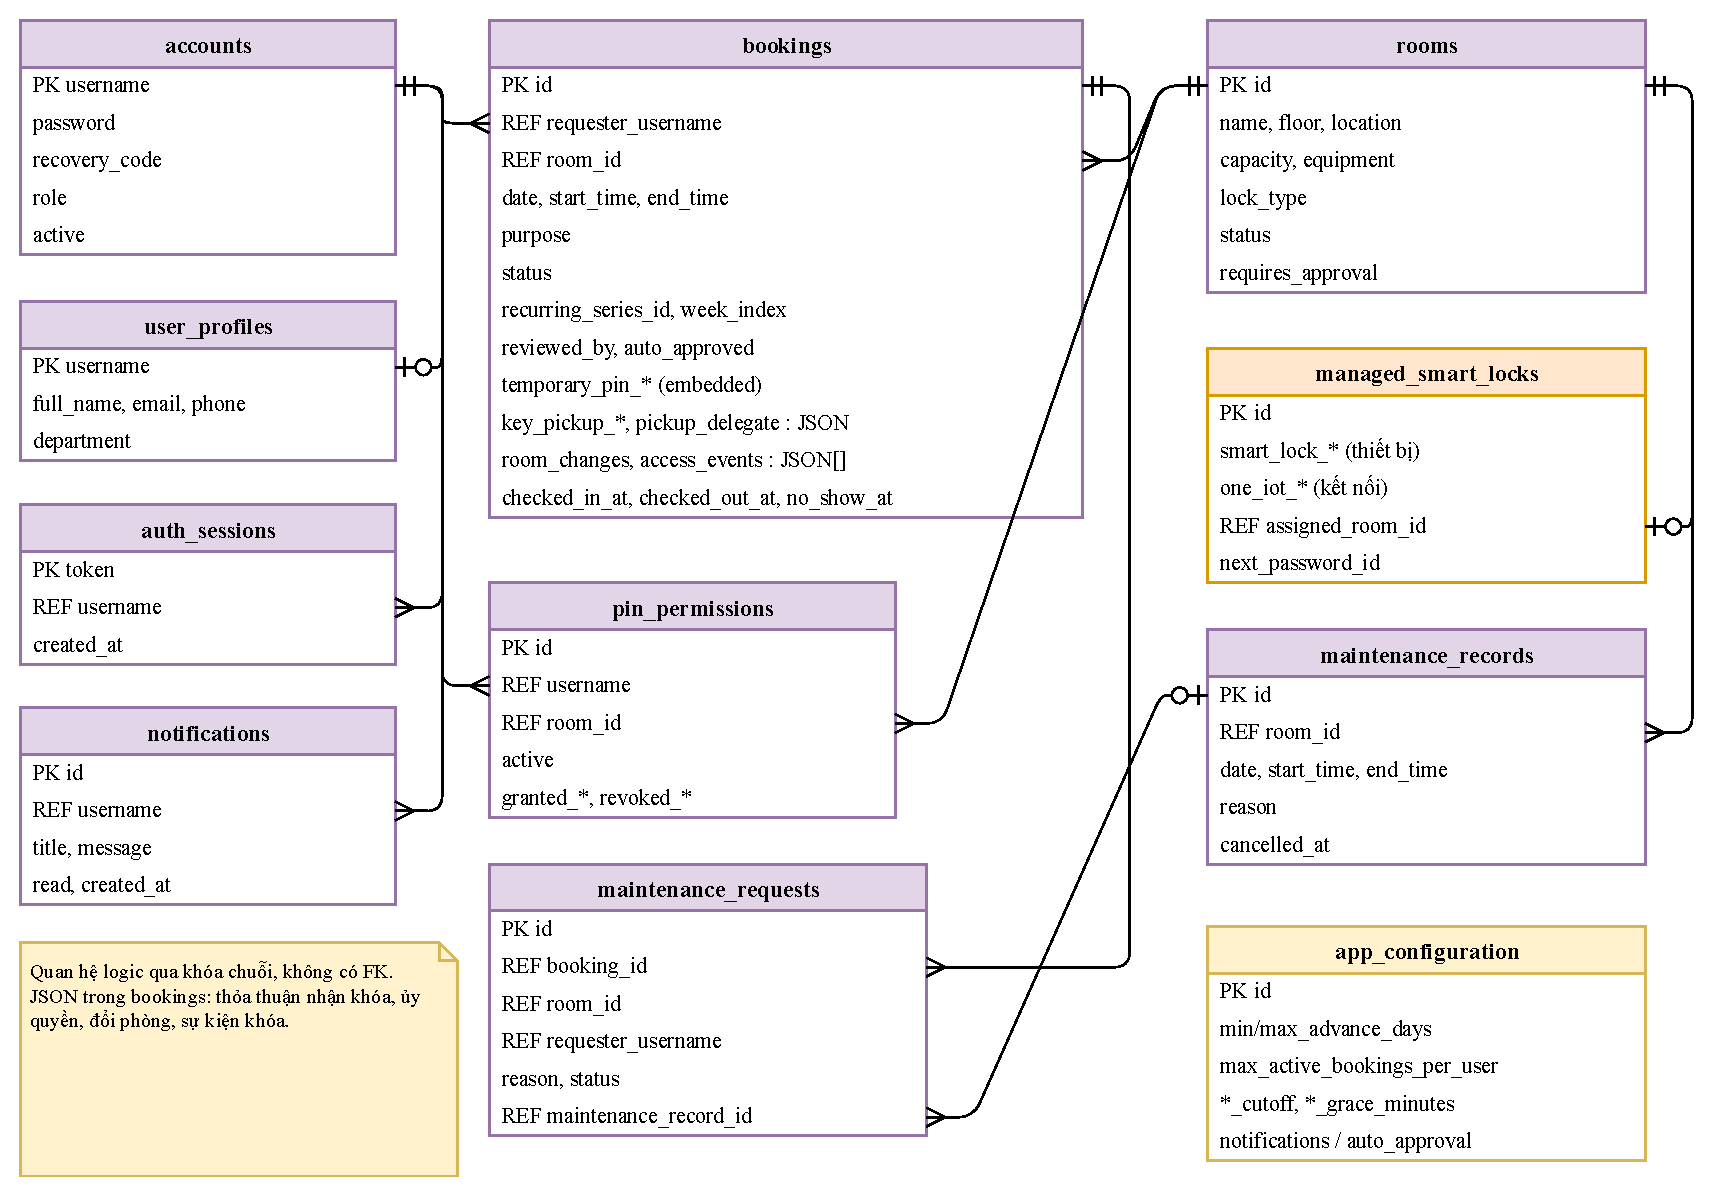
\includegraphics[width=.98\linewidth,height=.85\textheight,keepaspectratio]{Hinhve/design/17_er_diagram.pdf}
\caption{Mô hình thực thể và quan hệ logic của RoomHub}\label{fig:erd}
\end{figure}
\clearpage
\end{landscape}

\section{Quy trình tái lập kỹ thuật}\label{sec:technical-reproduction}
\subsection{Đóng gói Release trên macOS/Linux}
Các lệnh sau thực hiện tại \code{code/booking_classroom/}, sau khi cấu hình JDK/SDK, chọn nguồn dữ liệu và chạy \cmd{npm ci}. Bước bundle đưa JavaScript và tài nguyên vào APK trước khi Gradle đóng gói:
\begin{Verbatim}[fontsize=\small,frame=single,breaklines=true]
mkdir -p android/app/src/main/assets
node node_modules/react-native/cli.js bundle \
  --platform android --dev false --entry-file index.js \
  --bundle-output android/app/src/main/assets/index.android.bundle \
  --assets-dest android/app/src/main/res
cd android
sh ./gradlew assembleRelease
cd ..
\end{Verbatim}

Cài APK và mở ứng dụng theo mục 4.7. Trên Windows, script \cmd{npm run build:android:release} thực hiện các bước bundle và Gradle tương ứng.

\subsection{Tái lập kiểm thử}\label{sec:test-reproduction}
Các bộ ứng dụng, quality, quyền thông báo và kiểm tra tĩnh chạy từ thư mục ứng dụng; dữ liệu kết quả được lưu riêng cho từng bộ:
\begin{Verbatim}[fontsize=\small,frame=single,breaklines=true]
npm test -- --runInBand
npx jest --config quality-tests/jest.config.js --runInBand
npx jest --config ../../docs/reports/final/LTUD/minh_chung/kiem_thu/jest.permission.config.cjs --runInBand
npx tsc --noEmit
npm run lint
\end{Verbatim}

Kiểm thử backend dùng \cmd{mvn test} tại \code{code/booking-server/}. Môi trường, dữ liệu và kết quả thực nghiệm Android được lưu trong hồ sơ kiểm thử \cite{currenttests}; lệnh ADB và vị trí ảnh/XML đi kèm hồ sơ.
